\section{基于树与规则的分类}
\label{sec:classification-trees}

有些类别关系由局部条件决定：先检查一个特征，只有条件不满足时才需要查看另一个特征。例如图\ref{fig:classification-tree-partition}中的教学分类规则，在左半区域一律输出类1，在右半区域才由第二个坐标决定类别。一个全局线性得分不能精确表达整片区域中的这两段分界。分类树沿用第\ref{sec:classic-overview-trees-rules}节的条件分支，把输入逐步送入不同区域，再在叶节点输出类别或类别比例；路径中的先后测试使后续条件只在相应区域生效。

沿用训练集$D_n=\{(\bm{x}_i,y_i)\}_{i=1}^n$，其中输入有$d$个特征，$y_i\in\{1,\ldots,C\}$。本节允许特征是数值型或类别型，用$D\subseteq D_n$表示到达某个节点的训练样本。建树需要同时确定测试特征、阈值或取值分组，以及叶节点的输出，并非只估计一组预先固定的数值参数。常见做法是在当前节点选择一个能改善类别划分的测试，再递归处理各个子集；为避免把偶然差异也变成分支，还要限制生长或在生长后\term{剪枝}（pruning），即删除缺少预测收益的子树。

图~\ref{fig:classification-tree-partition}把同一个分类器分别画成区域和条件树。在$[0,1]^2$内，$x_1\leq0.5$的输入直接判为类1；其余输入继续检查$x_2$，不超过$0.55$时判为类2，否则判为类1。左图的水平分界只出现在右半区域，正对应右图中第二次测试只对第一个条件不成立的输入执行。这说明树中的路径不仅记录有哪些条件，也规定条件在哪个区域生效。

\begin{figure}[htbp]
  \centering
  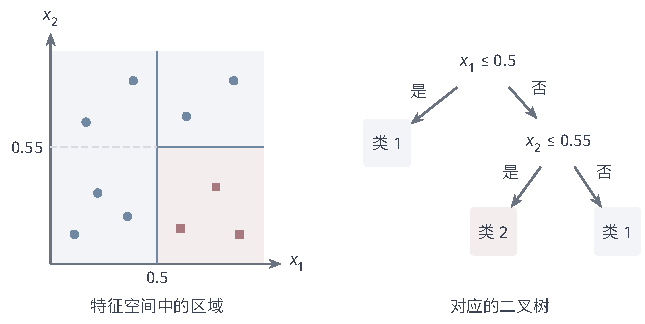
\includegraphics[width=109.241mm]{figures/04-classic-models/00-shared/tikz/classification-tree-partition/figure.pdf}
  \caption{二维分类的教学构造。左图为归一化特征空间$[0,1]^2$中的区域划分，圆点表示类1，方点表示类2；右图为产生同一划分的条件树。根节点检查$x_1\leq0.5$，仅在其“否”分支上继续检查$x_2\leq0.55$。点的位置与分裂阈值均为人为设定，不代表真实数据实验。}
  \label{fig:classification-tree-partition}
\end{figure}

不同树算法的主要差异落在三个问题上：怎样评价一次分裂，允许什么样的分支结构，怎样控制树的大小。ID3提供了信息增益驱动的基本构造，C4.5扩展其评分和数据处理方式；CART则采用统一的二叉划分与子树选择框架；LMT与CTree分别在叶内嵌入线性模型、用统计检验控制分裂；规则学习另起一条直接归纳条件列表的路线。

\subsection{ID3}
\label{sec:classification-id3}

要决定先检查哪个特征，需要比较“检查前还分不清多少类别”和“检查后还分不清多少类别”。这需要一个数来衡量一个节点里的类别“混得有多乱”。直觉上，如果节点里全是同一类，已经没有任何不确定，这个数应为零；如果各类各占一半，随便取一个样本很难猜中类别，这个数应取最大值。信息论用\term{熵}（entropy）给出这样一个量：它衡量在该节点的类别比例下，随机猜一个样本类别时平均还需要多少信息量（以2为底时单位是比特）。ID3（Iterative Dichotomiser 3）选择让这个不确定性下降最多的特征，再在各分支上重复同一过程。Quinlan在1986年的论文中将ID3追溯到Hunt等人的概念学习系统（Concept Learning System, CLS）：CLS向前考察若干层候选树，按测量与误分类代价选择测试；ID3则改用信息驱动的局部评价。这一变化把建树中的“先测什么”落实为当前节点上可计算的信息增益比较，优化范围限定在当前节点的候选测试。本节采用以离散特征、信息增益和不作后剪枝为设定的基本ID3\scite{quinlan1986trees}。

\subsubsection{模型结构}
\label{sec:classification-id3-structure}

在节点样本集$D$上，记$p_c(D)$为类别$c$的样本比例。采用以2为底的对数，熵为
\begin{equation}
  H(D)=-\sum_{c=1}^{C}p_c(D)\log_2 p_c(D),
  \label{eq:classification-entropy}
\end{equation}
其中约定$0\log_2 0=0$：它在节点只含一类时为零，各类越均匀熵越大。对第$j$个离散特征，令$V_j$为其可能取值集合，$D_{j,v}=\{(\bm{x}_i,y_i)\in D:x_{i,j}=v\}$。该特征的\term{信息增益}（information gain）是分裂前后熵的减少量：
\begin{equation}
  \operatorname{Gain}(D,j)
  =H(D)-\sum_{v\in V_j}\frac{|D_{j,v}|}{|D|}H(D_{j,v}).
  \label{eq:classification-information-gain}
\end{equation}
空子集对求和的贡献定义为零。这里必须按子集大小加权，否则只有一个样本的小分支会与包含大部分样本的分支同样重要。

ID3用选中的特征建立一个内部节点，每个取值对应一个分支。叶节点保存到达该处的类别计数，并通常输出多数类；类别计数相同时使用预先固定的平局规则。这样得到的是分段常值分类器：同一叶区域内的所有输入具有相同预测。叶节点也可报告类别频率，但少量样本上的频率不应被直接理解为可靠的概率估计。

信息增益把分裂选择变成了可计算的局部比较，却有\term{多值偏差}（multivalued attribute bias）：取值很多的特征更容易把训练样本分成纯净的小组。若每条记录的编号都不同，用编号分裂会使所有子节点熵为零，增益达到$H(D)$，但对一个新编号几乎没有帮助。

\subsubsection{参数学习}
\label{sec:classification-id3-learning}

\paragraph{信息增益与递归训练}
从根节点的$D_n$出发，算法计算所有可用特征的信息增益，选择最大者，再分别对其子集递归建树。离散特征已经按取值完全展开后，同一路径上不必再次使用它。若当前样本全部同类，就生成该类叶节点；若可用特征耗尽而标签仍不一致，就输出当前多数类。对训练时未出现的分支，可以保留以父节点多数类为输出的回退叶节点，使预测规则对新输入仍有定义。

\paragraph{局部评分的搜索边界}
每次选择只依据当前节点，因而这是\term{贪心搜索}（greedy search）：接受眼前收益最大的分裂，不回头枚举所有可能的整棵树。基本ID3不在建树后再作剪枝；限制最大深度、最小叶样本数或最小增益，属于另外加入的生长控制。尤其是“增益为零就停止”也会改变基本搜索行为：在异或关系中，单个特征的增益可能为零，而连续两次测试可以完全分开类别。停止规则既能减少无效分裂，也可能阻止发现特征交互。

离散特征在同一路径最多使用一次，因而基本递归会结束；这不表示信息增益贪心找到了所有树中的最小错误解。多条路径能组合特征条件，但特征记录相同而标签不同的样本，仍只能由同一叶的类别比例概括。

\subsection{C4.5}
\label{sec:classification-c45}

ID3的基本构造已经能从离散特征递归建树，但前面用记录编号的例子说明，信息增益会偏爱把训练样本切得很细的特征。实际记录还常有连续测量值和缺失字段：不能为每个长度值都建立一条新分支，也不能遇到未知值就让预测失去定义。让树处理这些数据，需要同时调整测试评分、阈值选择与缺失记录的传递方式。

Quinlan在1993年的专著中给出了C4.5的完整程序体系。它沿用ID3的递归构造，用增益率抑制部分多值偏差，通过阈值测试处理连续变量，并以分数权重传递缺失记录；树长成以后，再用错误估计剪枝和规则提取控制结构。以下分别说明这些机制如何工作\scite{quinlan1993c45}。

\subsubsection{模型结构}
\label{sec:classification-c45-structure}

多值特征容易得到大增益，是因为它本身就把数据切得很细。C4.5用\term{信息增益率}（gain ratio）比较“类别信息的增加”与“产生这些分支所需的划分信息”。设测试$a$把$D$分成$D_1,\ldots,D_b$，令$q_v=|D_v|/|D|$，则
\begin{align}
  \operatorname{SplitInfo}(D,a)
  &=-\sum_{v=1}^{b}q_v\log_2 q_v,
  \label{eq:classification-split-information}\\
  \operatorname{GainRatio}(D,a)
  &=\frac{\operatorname{Gain}(D,a)}
          {\operatorname{SplitInfo}(D,a)}.
  \label{eq:classification-gain-ratio}
\end{align}
这里的信息增益仍按式\eqref{eq:classification-information-gain}计算，只把按特征取值划分替换为测试$a$的各个结果。分母为零意味着没有真正划分，不能参与比值比较。

小分母会改变增益率的排序：只分离少量样本的测试具有较小的划分信息，微小信息增益也可能得到较大比值。C4.5先计算候选的平均信息增益，再在增益不低于平均值的测试中比较增益率。这个启发式筛选限制依靠小分母取胜的候选，实际预测价值仍由独立验证评价。

\subsubsection{参数学习}
\label{sec:classification-c45-learning}

在增益率筛选下递归生长：每次生成各特征的有效测试，保留增益不低于平均者，选增益率最大者分裂，缺失值按后文约定处理，空分支接父节点多数类叶。算法~\ref{alg:classification-c45}突出这些版本共有的建树骨架，把阈值评价留在候选测试生成步骤中\scite{quinlan1996continuous}。

\begin{algorithm}[C4.5的递归生长与后剪枝]
  \label{alg:classification-c45}
  \begin{algorithmic}[1]
    \Require 节点样本$D$，可用特征集合$F$，停止及剪枝设置
    \Ensure 剪枝后的分类树
    \Function{Grow}{$D,F$}
      \If{$D$全部同类，或样本量不足，或$F$为空}
        \State \Return 以$D$中多数类为输出的叶节点
      \EndIf
      \State 生成各特征的有效测试，连续特征同时选择阈值
      \State 计算各测试的增益；缺失值按正文约定处理
      \If{没有有效测试，或最大增益不为正}
        \State \Return 以$D$中多数类为输出的叶节点
      \EndIf
      \State 求候选测试的平均增益$\bar g$
      \State 保留增益不低于$\bar g$且划分信息为正的测试
      \State 选择其中增益率最大的测试$a$，建立节点$T$
      \For{测试$a$的每个结果$v$}
        \State 得到相应的子集$D_v$及子问题的特征集合$F_v$
        \If{$D_v$为空}
          \State 将$D$的多数类叶节点接到分支$v$
        \Else
          \State 将$\Call{Grow}{D_v,F_v}$接到分支$v$
        \EndIf
      \EndFor
      \State \Return $T$
    \EndFunction
    \State $T\gets\Call{Grow}{D,F}$
    \State 自底向上比较子树与简化方案的悲观错误估计
    \State \Return 剪枝后的$T$
  \end{algorithmic}
\end{algorithm}

\subsubsection{支持连续输入：阈值测试}
离散特征可以按取值作多路分裂；连续特征则使用$x_j\leq t$与$x_j>t$的二路测试。候选阈值来自排序后相邻不同取值之间，且分裂后必须满足最小子节点样本量等限制。连续特征在某次分裂后仍可在后代节点使用，因为同一数值轴上可能需要多个阈值。

C4.5各版本对阈值的评价略有区别。较早版本按增益率选择阈值；Quinlan在1996年的修订中先按信息增益选择连续特征的阈值，再扣除搜索阈值所需的描述长度代价，参与特征之间的增益筛选和增益率比较。若有$q$个候选切分位置，这项逐样本惩罚形如$\log_2 q/|D|$，用来抵消“可试阈值更多”带来的选择优势。

\subsubsection{支持缺失字段：评分与分数路由}

\paragraph{含缺失字段的候选评分}
缺失值需要在评分和路由中保留不确定性。当前节点的记录可能已经带有分数权重，因此下面用权重之和替代样本个数。记节点总权重为$W>0$，对测试$a$具有已知取值的记录总权重为$W_{\mathrm K}$，各个已知结果分支的权重为$W_v$，其中$v=1,\ldots,b$且$\sum_vW_v=W_{\mathrm K}$。原来的已知比例就是$q_{\mathrm{known}}=W_{\mathrm K}/W$；这里未知的是测试所用的属性值，训练记录的类别标签仍然已知。

先只用属性已知的记录计算类别熵。用这些记录的加权类别比例得到分裂前的熵$H_{\mathrm K}$，用第$v$个已知结果中的加权类别比例得到分支熵$H_v$。当$W_{\mathrm K}>0$时，先在已知部分计算熵下降，再按它在整个节点中的占比缩小：
\begin{align}
  \operatorname{Gain}_{\mathrm K}
    &=H_{\mathrm K}-\sum_{v=1}^b
        \frac{W_v}{W_{\mathrm K}}H_v,\notag\\
  \operatorname{Gain}(D,a)
    &=\frac{W_{\mathrm K}}{W}\operatorname{Gain}_{\mathrm K}.
  \label{eq:classification-c45-missing-gain}
\end{align}
分支类别比例和这里的子熵加权都以已知部分为范围；它们不能把未知属性当成某个已知结果。没有已知记录的结果，其求和项按零贡献处理。上述式子给出熵下降的缺失修正；若所用版本还要扣除连续阈值的描述长度代价，仍按前面的约定处理。

增益率的分母则衡量整个节点的测试结果有多少不确定性。各个已知结果占$W_v/W$，未知部分占$1-W_{\mathrm K}/W$，因此
\begin{equation}
  \begin{aligned}
    \operatorname{SplitInfo}(D,a)
      &=-\sum_{v=1}^b\frac{W_v}{W}
          \log_2\frac{W_v}{W}\\
      &\quad-\left(1-\frac{W_{\mathrm K}}{W}\right)
          \log_2\left(1-\frac{W_{\mathrm K}}{W}\right).
  \end{aligned}
  \label{eq:classification-c45-missing-split-info}
\end{equation}
零权重项仍按$0\log_2 0=0$处理。这一步把未知部分单列为一组，只为计算测试评分，并不在预测树上增加一个“未知”结果分支。

例如，构造10条等权训练记录，其中8条的测试值已知：6条类1记录进入左分支，2条类2记录进入右分支。另外2条记录只有该测试值未知，其标签分别为类1和类2。因此$W=10$、$W_{\mathrm K}=8$、$W_{\mathrm L}=6$、$W_{\mathrm R}=2$。已知部分的类别比例为$3/4$和$1/4$，两个已知分支都是纯节点，于是
\[
  \begin{aligned}
    H_{\mathrm K}
      &=-\frac34\log_2\frac34-\frac14\log_2\frac14
        \approx0.8113,\\
    \operatorname{Gain}(D,a)
      &=\frac8{10}H_{\mathrm K}\approx0.6490.
  \end{aligned}
\]
这里没有用全节点的$7:3$类别计数替代已知部分的$6:2$计数。划分信息使用的是三个结果组的比例$0.6,0.2,0.2$，故
\[
  \begin{aligned}
    \operatorname{SplitInfo}(D,a)
      &=-0.6\log_2 0.6-2(0.2\log_2 0.2)
        \approx1.3710,\\
    \operatorname{GainRatio}(D,a)
      &\approx0.6490/1.3710\approx0.4734.
  \end{aligned}
\]
熵和信息增益的单位为比特，增益率是两者的比值。

\paragraph{训练与预测的分数路由}
选定测试以后，才决定未知记录如何进入子树。每条权重为$w$的未知记录，向第$v$个已知结果分支传递$wW_v/W_{\mathrm K}$的权重；这些权重之和仍为$w$，记录的类别标签不变。上述例子中，每条未知记录分别给左右分支贡献$6/8=0.75$和$2/8=0.25$的权重。因此左节点的类1、类2权重变为$6.75,0.75$，右节点变为$0.25,2.25$，两个节点总权重分别为$7.5$和$2.5$。后续熵、类别计数和多数类都使用这些分数权重。

评分时用节点总权重$W$归一化测试结果，路由时却用已知总权重$W_{\mathrm K}$归一化已知分支。因而评分中的$0.6,0.2,0.2$不能换成路由比例$0.75,0.25$，也不能用分流后的子节点权重重新定义这次分裂的已知结果比例。若$W_{\mathrm K}=0$，就没有可用来估计分支比例的已知记录，应把该测试视为无效候选，而不能继续除法；划分信息为零的测试同样不能参加增益率比较。预测遇到缺失值时，也按已知分支的相对权重综合子树输出。

\subsubsection{简化预测结构：后剪枝与规则提取}
树生长完成后，C4.5采用\term{悲观错误剪枝}（pessimistic error pruning）：训练误差倾向于低估新样本错误，因而以二项错误计数的上置信估计作修正，比较保留子树与折叠成多数类叶节点的估计错误数。若简化方案不更差，就可以删除该子树；完整实现还可考察用某个子树提升替代当前分支。置信设置控制剪枝强度，这一自适应建树后的估计用于启发式模型选择，整树的样本外错误仍通过验证或测试数据评价。

树也可以转成规则：每条根到叶路径的测试构成规则前件，叶类别作为后件，再尝试删除不必要条件并筛选规则。未经简化的路径规则继承树的区域划分；条件删除以后可能产生重叠，因此规则系统还必须规定冲突处理和默认预测。这种转换并非只把树的文字抄成一份无序清单。

连续阈值形成轴对齐分区，增益率改变的是搜索偏好，并不会把一条坐标边界变成斜线。缺失记录按权重分流后，不能再用“每次样本个数严格下降”证明停止；实现还需最小有效权重、深度等生长限制。生成测试、处理缺失值、剪枝和规则提取是相互配套的学习过程，不能仅用增益率概括整个C4.5。

\subsection{CART}
\label{sec:classification-cart}

另一种组织树的方法是把每次测试都限定成二选一，再统一研究大树中应保留哪些子树。\term{分类与回归树}（classification and regression trees, CART）采用这一框架；Breiman、Friedman、Olshen与Stone在1984年的专著中将树的构造、最优剪枝与统计性质放在同一体系中讨论。其中，代价复杂度剪枝把“怎样长出一棵大树”与“最终保留多大的子树”分开：生长阶段比较局部分裂，剪枝阶段形成候选子树序列，再用验证选择规模。因此，CART与ID3的区别不只是换一个不纯度指标，还涉及分支结构与整树选择。这里关注分类树；第\ref{sec:regression-cart}节的回归CART复用递归二分与代价复杂度剪枝，但按响应损失选择分裂并在叶内输出数值，本节则按类别不纯度或误分类代价分裂并输出类别标签或类别比例\scite{breiman1984cart}。

\subsubsection{模型结构}
\label{sec:classification-cart-structure}

CART分类树通常用\term{基尼不纯度}（Gini impurity）评价节点中类别的混杂程度：
\begin{equation}
  G(D)=1-\sum_{c=1}^{C}p_c(D)^2.
  \label{eq:classification-gini}
\end{equation}
它也等于从节点经验类别分布独立抽取两个标签时，两者不同的概率。对于产生左右子集$D_{\mathrm{L}}$和$D_{\mathrm{R}}$的测试$a$，比较
\begin{equation}
  \Delta G(D,a)=G(D)
  -\sum_{v\in\{\mathrm{L},\mathrm{R}\}}
  \frac{|D_v|}{|D|}G(D_v).
  \label{eq:classification-gini-decrease}
\end{equation}
基尼与熵都鼓励子节点变纯，但并不总给出相同的排序。基尼计算省去对数运算，整棵树的训练成本还包含阈值搜索与数据访问。

对连续特征，二分测试仍是阈值比较；对类别特征，测试可写成$x_j\in S$与$x_j\notin S$，其中$S$是部分取值组成的集合。寻找这个集合本身也是搜索问题，候选分组数随取值数增加，搜索成本需要计入建树预算。统一的二叉结构便于遍历和剪枝，但可能用多层测试表达一棵多路树的一次分裂。

\subsubsection{参数学习}
\label{sec:classification-cart-learning}

\paragraph{二叉树生长}
生长阶段反复选择基尼下降最大的有效二分测试，直到满足生长限制，得到一棵较大的树$T_0$。

\paragraph{剪枝与规模选择}
随后进行\term{代价复杂度剪枝}（cost-complexity pruning）：不再逐个比较局部增益，而是在$T_0$的候选子树中平衡拟合误差和叶节点数。令$L(T)$为树$T$的叶节点集合，$\hat c_\ell$为叶$\ell$的预测类别，定义
\begin{align}
  \widehat R(T)
  &=\frac{1}{n}\sum_{\ell\in L(T)}
    \sum_{(\bm{x}_i,y_i)\in D_\ell}
    \mathbb{1}\{y_i\neq\hat c_\ell\},
  \label{eq:classification-cart-empirical-risk}\\
  J_\alpha(T)&=\widehat R(T)+\alpha|L(T)|,
  \qquad \alpha\geq0.
  \label{eq:classification-cart-cost-complexity}
\end{align}
这里$\widehat R(T)$采用全训练集上的误分类比例，使不同子树的误差具有共同尺度。有些软件把叶不纯度的加权和作为剪枝代价；使用其参数时需要核对具体定义，再按该尺度解释$\alpha$。

剪枝路径可以由\term{最弱环节剪枝}（weakest-link pruning）生成。设内部节点$t$以下的子树为$T_t$，把它折叠成一个叶节点后，该区域对全训练集误差的贡献为$\widehat R(t)$；保留时贡献为$\widehat R(T_t)$。两种方案的代价相等时，
\begin{equation}
  \alpha_t=
  \frac{\widehat R(t)-\widehat R(T_t)}
       {|L(T_t)|-1}.
  \label{eq:classification-weakest-link}
\end{equation}
分子是折叠后增加的训练错误，分母是删去的叶数，因而$\alpha_t$衡量“每少保留一个叶节点要付出多少误差”。剪去最小$\alpha_t$对应的分支，再重新计算，就得到从大树到根叶节点的嵌套序列。若某些分支增加叶数却不降低误分类率，可先在$\alpha=0$时合并；临界值处可能有多个最优子树，按一致的最小子树约定处理平局。

对每个$\alpha$，上述序列包含相应的最优剪枝子树，最优性范围限定为给定$T_0$的剪枝子树。实际需要用验证集或交叉验证选择$\alpha$；交叉验证时，在各训练折内独立生长和剪枝，再评价对应验证折。

图~\ref{fig:classification-cart-pruning}用一棵教学树展示这一序列。设最弱环节剪枝依次得到四棵嵌套子树：$T_0$有$4$个叶、训练误分类率$\widehat R=0.10$；$T_1$有$3$个叶、$\widehat R=0.12$；$T_2$有$2$个叶、$\widehat R=0.16$；根叶$T_3$有$1$个叶、$\widehat R=0.30$。相邻两棵代价相等$\widehat R_i+|L_i|\alpha=\widehat R_{i+1}+|L_{i+1}|\alpha$的临界值为$\alpha_k=(\widehat R(T_{k+1})-\widehat R(T_k))/(|L(T_k)|-|L(T_{k+1})|)$，代入得$\alpha=0.02$、$0.04$、$0.14$：最优子树在分段区间$[0,0.02)$、$[0.02,0.04)$、$[0.04,0.14)$、$[0.14,\alpha_{\max})$上依次为$T_0$、$T_1$、$T_2$、$T_3$，代价$J_\alpha(T)$对$\alpha$的下包络（图\ref{fig:classification-cart-pruning}(a)中粗线）就在这些切点切换。

每段内训练误差取该段子树的$\widehat R(T_k)$、不随$\alpha$变化（图\ref{fig:classification-cart-pruning}(b)灰横线），随剪枝单调上升；教学构造的验证误差在四段上依次为$0.22$、$0.19$、$0.18$、$0.33$，每段都高于同段训练误差并在$T_2$段取最小，于是该段内任意$\alpha$都对应$T_2$，取代表值$\alpha^*=0.04$。

\begin{figure*}[tbp]
  \centering
  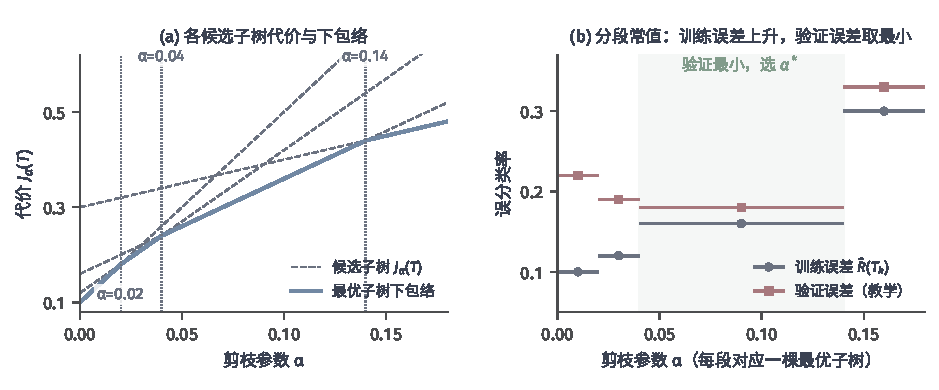
\includegraphics[width=159.0mm]{figures/04-classic-models/00-shared/matplotlib/classification-cart-pruning/figure.pdf}
  \caption{代价复杂度剪枝的教学序列。(a)四棵候选子树的代价$J_\alpha(T)=\widehat R(T)+\alpha|L(T)|$随$\alpha$上升，虚线为各子树、粗线为下包络，竖线标出相邻子树代价相等的切点$\alpha=0.02,0.04,0.14$；(b)最优子树随$\alpha$分段常值——每段一条水平线给出该段子树的训练误差$\widehat R(T_k)$与教学验证误差（每段高于同段训练误差），绿色阴影段验证误差最小（$0.18$），取代表值$\alpha^*=0.04$。数据为明示的教学构造，不代表真实实验。}
  \label{fig:classification-cart-pruning}
\end{figure*}

\subsubsection{理论分析}
\label{sec:classification-cart-theory}

\paragraph{固定树的剪枝最优性}
上述最弱环节路径中的最优性限定在已长出的$T_0$的剪枝子树，不能扩展为所有可构造树中的最优性。

\paragraph{结构搜索与统计评价}
只用单坐标阈值时，叶区域仍由坐标区间的交组成；增加叶数可以细化分区，却不能恢复输入或允许测试根本没有保留的类别信息。最终树的大小、停止条件和阈值选择须在独立于拟合过程的验证中评价。

\subsubsection{支持缺失主测试：替代分裂}
\label{sec:classification-cart-surrogate}
预测还要规定主测试字段缺失时如何分支。CART的\term{替代分裂}（surrogate split）寻找其他特征测试，按它们复现主分裂结果的程度选择替代：先统计每个候选测试与主测试把样本分到同一侧的比例，取复现程度最高者作为第一替代，再依次排列。主字段缺失时，按排名依次使用第一个字段可用的替代分裂；全部替代都缺失时，才按叶内多数类或类别权重直接判决。类别权重和误分类代价也可以改变生长与叶预测。具体实现采用哪些机制，需要与数据处理方式一同检查。

误拦正常邮件与漏放垃圾邮件可能有不同代价。令$L_{a,c}$为真实类别$c$却输出$a$时的代价，在叶$\ell$内用训练类别比例$\hat p_{\ell,c}$估计局部分布，就应选择
\[
  \hat c_\ell=\argmin_a\sum_{c=1}^C L_{a,c}\hat p_{\ell,c}.
\]
零一代价时它退化为多数类。若训练目标也按这些代价评价，生长评分和剪枝误差应采用相应口径；只在最后改阈值与从建树起使用加权误差，不是同一个学习过程。代价由实际决策问题确定，树的参数仍由训练数据估计，并用匹配代价的验证指标选择规模。非对称代价决策的一般框架见第\ref{sec:classification-cost-decision}节。

\subsection{逻辑模型树（LMT）}
\label{sec:classification-lmt}

常数叶用一个概率向量概括区域中的全部输入；若同一区域内的概率仍随特征变化，可以保留树的划分，改变叶节点如何预测。\term{逻辑模型树}（logistic model tree, LMT）在每个叶区域内使用Logistic回归，即用特征的线性得分表示类别对数几率，再转成类别概率。这样，树负责不同区域之间的结构变化，叶模型负责区域内部随特征变化的概率。Landwehr、Hall与Frank的2005年期刊论文基于其2003年会议工作，结合C4.5分裂与CART剪枝形成树结构，并通过LogitBoost逐步拟合逻辑模型。在后代节点继续细化祖先模型，可以避免每个小叶都从零估计全部系数\scite{landwehr2005lmt}。

\subsubsection{模型结构}
例如在二分类叶区域$\ell$内，LMT可输出
\begin{equation}
  \hat p_\ell(y=1\mid\bm{x})
  =\frac{1}{1+\exp[-(\bm{w}_\ell^\top\bm{x}+b_\ell)]},
  \label{eq:classification-lmt-leaf}
\end{equation}
其中$\bm{w}_\ell\in\mathbb{R}^d$和$b_\ell\in\mathbb{R}$是叶模型的系数。概率在单个叶区域内部平滑变化，但跨越不同叶的边界时仍可能跳变，也不自动具有良好的校准性质。模型拟合、迭代次数选择和树剪枝共同增加训练成本，解释时也要同时阅读路径条件与叶模型系数。

\subsubsection{参数学习}

\paragraph{节点逻辑模型拟合}
训练逻辑模型时，不能把“叶中放一个Logistic回归”当成参数已经给定。LMT使用LogitBoost逐轮修正节点内的线性得分，其单轮修正就是二项对数损失对节点线性预测子的二阶展开（Newton配方）：按当前概率给曲率权重$v_i=p_i(1-p_i)$与修正工作响应$z_i=(y_i-p_i)/v_i$，再拟合加权最小二乘的线性修正项，将它加入得分并重新计算概率。以标签编码为0、1的二分类为例，当前样本概率为$0<p_i<1$时，$v_i=p_i(1-p_i)$表示按局部曲率缩放的拟合权重，$z_i=(y_i-p_i)/[p_i(1-p_i)]$表示按同一曲率缩放的拟合方向；它是供拟合增量$\Delta\beta$的工作响应，与第\ref{sec:classification-logistic-learning}节IRLS相比曲率权重$v_i$相同，只是不含当前得分$\eta_i$。写成矩阵形式，加权最小二乘的正规方程恰为$\tilde{\bm X}^{\top}\operatorname{diag}(v_i)\tilde{\bm X}\,\Delta\bm\beta=\tilde{\bm X}^{\top}(\bm y-\bm p)$，右端即负对数似然梯度$\tilde{\bm X}^{\top}(\bm p-\bm y)$取负号——因此节点$\bm\beta$的每一步Newton修正都是该加权Logistic目标在当前点的$-\bm H^{-1}\nabla L$步，并非另立一套损失。

原方法每轮比较单个特征上的简单线性回归，选择加权拟合误差较小的修正，因此最终得分仍是线性的。多分类时为各类拟合修正，并作中心化校正后，把类得分的指数归一化为概率；迭代次数通过交叉验证选择。

\paragraph{树结构与迭代数选择}
根节点先用全部训练样本拟合。分裂后，子节点继承父节点已有的得分函数，在进入该节点的样本上继续上述迭代，而非分别从零拟合互不关联的叶模型。C4.5式分裂继续决定数据怎样分组，CART式剪枝与验证决定保留哪些区域。这样，父节点学到的共同影响与子节点新增的局部影响共同形成预测；数值特征转换、缺失值处理以及迭代和剪枝选择也都属于训练流程。

\subsection{条件推断树（CTree）}
\label{sec:classification-ctree}

信息增益和基尼下降还面临另一种偏差：候选切分越多，越容易偶然找到一个高分切分。打个比方，掷一枚均匀硬币很多次，总可能出现某次连续正面特别多；同样，一个有很多取值的特征即使与类别毫无关系，也更容易因为偶然波动在训练集上切出很纯的子群。直接比较所有特征的得分，会系统性地偏向这种“候选机会更多”的特征。\term{条件推断树}（conditional inference tree, CTree）对症下药，把“先选哪个特征”与“再在该特征上怎样切分”分成两步，并在选特征时用统计检验回答：“观察到的关联，有没有可能只是有限样本里的偶然？”Hothorn、Hornik与Zeileis在2006年的框架中用条件置换分布评价特征与响应的关联\scite{hothorn2006ctree}。

\subsubsection{模型结构}
要判断某个字段显示的关联是否可能只是有限样本的偶合，需要建立“没有这种关联时，评分会怎样波动”的比较基准。在当前节点里，先固定全部输入值和各类标签的个数，再把这些标签在记录之间重新排列。若在相应无关联原假设下，交换标签位置不会改变这些排列的概率，也就是标签位置具有可交换性，那么这些排列就给出同一关联统计量在原假设下可能出现的取值。所谓条件置换分布，就是在这些已经固定的信息下，由标签位置的排列得到的比较分布；每次仍对同一字段计算同一统计量，不是打乱字段后重新训练另一棵树。

只为说明这个基准，考虑4条记录上的一个预先给定二值字段$\bm z=(0,0,1,1)$，临时把两类标签编码为0和1，观察到$\bm y=(0,0,1,1)$。用两组正类比例之差的绝对值作为关联统计量：
\[
  T=\left|\frac{y_1+y_2}{2}-\frac{y_3+y_4}{2}\right|.
\]
当前$T=1$，这个字段完全分开了两类。固定两个0和两个1后，标签共有$\binom42=6$种不同排列：正向或反向完全分开的2种排列给出$T=1$，其余4种给出$T=0$。因此，在这个无关联的排列基准下，“至少和当前一样极端”的比例为$2/6=1/3$，而不是零。小样本中一次纯净的分组并不自动给出很强的关联证据。这个教学例只解释置换比较的含义，CTree的具体关联统计量按其框架与实现规定。

当统计量越大表示关联越强时，原假设下出现当前或更大统计量的概率就是相应的$p$值（$p$-value）；它不是原假设为真的概率。把不同字段的关联评分转成各自原假设下的$p$值，才能在同一证据尺度上比较原始量纲、取值数不同的字段。同时检查多个字段会增加偶然选出小$p$值的机会，因此还需作相应的多重检验调整，不能把未经调整的最小$p$值直接当作整个节点的检验$p$值。否则，即使所有字段都无关联，也可能更频繁地被误判为有字段相关。

\subsubsection{参数学习}
CTree先检验当前节点中所有特征均与响应无关联的全局原假设；不能拒绝时停止，否则选择检验证据最强的特征，再为它寻找二分位置。通过这一共同检验尺度和多重检验控制，可以缓解不同取值数目带来的选择偏差。置换检验依赖原假设下的可交换性，渐近近似的精度也受样本量影响。检验控制当前节点是否继续分裂，全树的预测质量仍应在独立数据上评价。

检验驱动的生长也有搜索边界：四点异或在两层树中可被精确表示，但根节点的每个单坐标都与标签独立，单变量检验可能阻止继续分裂。检验决定当前节点是否继续搜索，并不改变候选树本来能够表示的关系。
